%% Concept figure (dissertation variant, Section 1.1): joint-trained grouping vs the modular PG-GAT pipeline.
%% Two stacked strips; the strip-(a) side note sits under the dashed box so the natural width stays within the
%% 441 pt text width of the thesis page (font \small = 9 pt; scale-to-\linewidth must stay >= 0.89 for the 8 pt floor).
%% Colour code as in the dissertation diagrams: red = trained in this work (frozen at inference),
%% blue = external pre-trained detector, grey = deterministic / data. Insets from fig_concept_insets.py
%% (COCO val2017 281759, HigherHRNet detections; K = 5, K-head 5, PGA 1.00).
%% Build (agent): pdflatex -output-directory=build_agent concept_modular.tex ; copy the PDF to ../concept_modular.pdf
%% Insets: ../concept_inset_ungrouped.pdf and ../concept_inset_grouped.pdf (fig_concept_insets.py, copied from the paper).
\documentclass[10pt,tikz,border=3pt]{standalone}
\usepackage[T1]{fontenc}
\usepackage{mathptmx}
\usepackage{amsmath,amssymb}
\usepackage{graphicx}
\usetikzlibrary{positioning,arrows.meta,calc,fit,backgrounds}

\begin{document}
\begin{tikzpicture}[
  font=\small,
  >={Stealth[length=2.2mm]},
  box/.style={draw=black!75, rounded corners=1.5pt, align=center, inner sep=3pt, minimum height=8mm, fill=white},
  data/.style={box, fill=black!5},
  ours/.style={box, draw=red!60!black, fill=red!10, thick},
  ext/.style={box, draw=blue!60!black, fill=blue!8, thick},
  det/.style={box, draw=black!55, fill=black!15},
  arr/.style={->, semithick, black!75},
  line/.style={semithick, black!75},
  dlbl/.style={font=\small\itshape, align=center},
  hdr/.style={font=\small\bfseries, align=left, anchor=north west},
]

%% ================= (a) joint-trained grouping (top strip) =================
\node[hdr] (ha) at (0,0) {(a) joint-trained grouping};
\node[data, anchor=north west, minimum width=14mm] (imga) at ($(ha.south west)+(0,-9mm)$) {image};
\node[ext, right=7mm of imga, text width=26mm] (bba) {detector backbone\\ \textnormal{\small (e.g.\ \mbox{HigherHRNet})}};
\node[ext, right=9mm of bba, yshift=5mm, text width=22mm] (hm) {keypoint heatmaps};
\node[ext, right=9mm of bba, yshift=-5mm, text width=22mm] (tag) {grouping head\\ \textnormal{\small (AE tags)}};
\coordinate (amid) at ($(hm.east)!0.5!(tag.east)$);
\node[data, right=7mm of amid, anchor=west, text width=16mm] (posea) {grouped\\ poses};
\draw[arr] (imga) -- (bba);
\draw[arr] (bba.east) -- ++(3.5mm,0) |- (hm.west);
\draw[arr] (bba.east) -- ++(3.5mm,0) |- (tag.west);
\draw[arr] (hm.east) -- ++(3mm,0) |- (posea.west);
\draw[arr] (tag.east) -- ++(3mm,0) |- (posea.west);
\begin{scope}[on background layer]
  \node[draw=blue!60!black, dashed, rounded corners=2pt, inner sep=2.5mm, fit=(bba)(hm)(tag)] (jt) {};
\end{scope}
\node[dlbl, blue!60!black, anchor=north] (jtnote) at (jt.south)
  {one network, trained together on one detector's features -\\
   grouping tied to its detector; swapping the detector means retraining the grouping};

%% ================= (b) modular grouping (bottom strip) =================
\node[hdr] (hb) at ($(imga.west |- jtnote.south)+(0,-6mm)$) [anchor=north west] {(b) modular grouping (this work)};
\node[ext, anchor=north west, text width=24mm] (hr) at ($(hb.south west)+(0,-3mm)$) {HigherHRNet};
\node[ext, below=2mm of hr, text width=24mm] (yolo) {YOLO11x-pose};
\node[ext, below=2mm of yolo, text width=24mm] (rtmo) {RTMO-L};
\coordinate (bus) at ($(hr.east)+(3mm,0)$);
\draw[line] (hr.east) -- (bus |- hr.east) -- (bus |- rtmo.east);
\draw[line] (rtmo.east) -- (bus |- rtmo.east);
\draw[line] (yolo.east) -- (bus |- yolo.east);
\node[data, text width=22mm, anchor=west] (kp) at ($(bus |- yolo.east)+(3mm,0)$)
  {keypoints only\\ $(x_i,y_i),\ t_i$\\ \textnormal{\small identities discarded}};
\draw[arr] (bus |- yolo.east) -- (kp.west);
\node[inner sep=0, right=5mm of kp, anchor=west] (ins1) {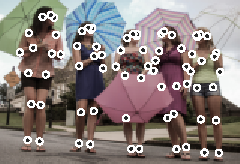
\includegraphics[height=16mm]{../concept_inset_ungrouped.pdf}};
\draw[arr] (kp.east) -- (ins1.west);
%% the interface
\coordinate (ifx) at ($(ins1.east)+(4.5mm,0)$);
\draw[dashed, thick, black!60] ($(ifx |- hr.north)+(0,4mm)$) -- ($(ifx |- rtmo.south)+(0,-2mm)$);
\node[dlbl, black!60, anchor=south] at ($(ifx |- hr.north)+(0,4.5mm)$) {detector-independent interface};
%% grouping module: PG-GAT in the middle row, k-means above, K-head below
\node[ours, text width=19mm, anchor=west] (pg) at ($(ifx |- yolo.east)+(8mm,0)$) {PG-GAT\\ \textnormal{\small (frozen)}};
\node[ours, below=2mm of pg, text width=19mm] (kh) {K-head\\ \textnormal{\small (frozen)}};
\node[det, above=2mm of pg, text width=19mm] (km) {$k$-means, $k=\hat K$};
\draw[arr] (ins1.east) -- (pg.west);
\draw[arr] (pg.south) -- (kh.north);
\draw[arr] (pg.east) -- ++(3mm,0) |- (km.east);
\node[dlbl, anchor=west] at ($(pg.east)+(3.5mm,0)+(0,5.5mm)$) {$\mathbf z_i$};
\draw[arr] (kh.west) -- ++(-3mm,0) |- (km.west);
\node[dlbl, anchor=east] at ($(pg.west)+(-3.5mm,0)+(0,5.5mm)$) {$\hat K$};
%% inset: the grouped result
\node[inner sep=0, anchor=west] (ins2) at ($(pg.east)+(9mm,0)$) {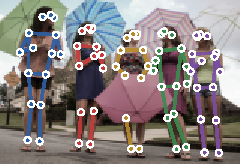
\includegraphics[height=16mm]{../concept_inset_grouped.pdf}};
\draw[arr] (km.east) -- ++(5mm,0) |- (ins2.west);
\node[dlbl, anchor=north] at ($(ins2.south)+(0,-0.5mm)$) {grouped poses};

%% ================= legend =================
\matrix[draw=black!40, rounded corners=1.5pt, inner sep=3pt, column sep=2.5mm, row sep=1mm,
        ampersand replacement=\&] (leg) at ($(hr.west |- rtmo.south)+(0,-13mm)$) [anchor=north west] {
  \node[ours, minimum height=4mm, minimum width=7mm, inner sep=1pt] {}; \& \node[align=left]{trained in this work, frozen at inference}; \&
  \node[ext, minimum height=4mm, minimum width=7mm, inner sep=1pt] {}; \& \node[align=left]{external pre-trained detector}; \&
  \node[det, minimum height=4mm, minimum width=7mm, inner sep=1pt] {}; \& \node[align=left]{no learned parameters}; \\
};
\end{tikzpicture}
\end{document}
